\documentclass[a4paper,12pt]{ctexart}

\usepackage{geometry}

\geometry{a4paper, left=2.5cm, right=2.5cm, top=2.5cm, bottom=2.5cm}

\usepackage{amsmath}

\usepackage{caption}

\usepackage{graphicx}

\usepackage{listings}

\usepackage{xcolor}

\usepackage{fontspec}

\usepackage{url}

\setmainfont{Microsoft YaHei}

\setkeys{Gin}{width=\textwidth, keepaspectratio}

\lstset{
	basicstyle=\footnotesize\ttfamily,
	frame=single,
	numbers=none,
	backgroundcolor=\color{gray!5},
	breaklines=true,
	breakatwhitespace=false,
	columns=flexible,
	xleftmargin=4pt,
	xrightmargin=4pt,
	breakindent=1em
}

\begin{document}
	
	\title{系统开发工具基础 第三周实验报告}
	\author{涂睿昕---25020007115}
	\maketitle
	
	\section{实验概述}
	本次实验为系统开发工具基础第三周课上实验，实验环境为VirtualBox中的Ubuntu虚拟机。本次完成四项课上实验：Python源码包构建与wheel分发、编程智能体测试驱动修复、协作沟通材料规范化改写、PyTorch线性回归训练循环调试补全。实验主要练习Python包构建工具build、虚拟环境隔离、测试驱动开发、工程化协作文档撰写、PyTorch模型训练流程，掌握源码打包、缺陷复现、问题规范化描述、深度学习训练循环排错的基本流程。
	
	\section{课上实验题目}
	\subsection{q09：从源码构建并在干净环境安装Wheel}
	\subsubsection{题目要求}
	创建最小Python命令行包，编写\texttt{pyproject.toml}配置；使用build工具从源码构建wheel分发包；新建干净虚拟环境，仅使用生成的wheel完成安装；切换到项目目录外部运行脚本入口命令，验证程序输出符合预期。
	
	\subsubsection{实现过程与关键命令}
	\begin{lstlisting}[language=bash]
		cd ~/sdt-course/week3/q09
		mkdir -p src/greetlab
		touch src/greetlab/__init__.py
		nano src/greetlab/cli.py
		nano pyproject.toml
		python3 -m build
		# 创建全新干净虚拟环境
		python3 -m venv venv-build
		source venv-build/bin/activate
		pip install --upgrade build
		python3 -m venv venv-test
		source venv-test/bin/activate
		ls dist/
		pip install ./dist/*.whl
		cd ..
		sdt-greet --name 25020007115
		deactivate
	\end{lstlisting}
	\texttt{src/greetlab/cli.py}核心代码：
	\begin{lstlisting}[language=Python]
		import argparse
		def main():
		p = argparse.ArgumentParser()
		p.add_argument("--name", required=True)
		a = p.parse_args()
		print(f"Hello, {a.name}!")
		
		if __name__ == "__main__":
		main()
	\end{lstlisting}
	\texttt{pyproject.toml}配置：
	\begin{lstlisting}
		[build-system]
		requires = ["setuptools>=68"]
		build-backend = "setuptools.build_meta"
		
		[project]
		name = "greetlab-25020007115"
		version = "0.1.0"
		
		[project.scripts]
		sdt-greet = "greetlab.cli:main"
	\end{lstlisting}
	
	\subsubsection{运行结果}
	执行\texttt{python3 -m build}后在dist目录生成对应的wheel文件；进入干净虚拟环境完成安装；切换到q09目录外部执行\texttt{sdt-greet --name 25020007115}，控制台输出\texttt{Hello, 25020007115!}，程序运行正常。
	
	\begin{figure}[htbp]
		\centering
		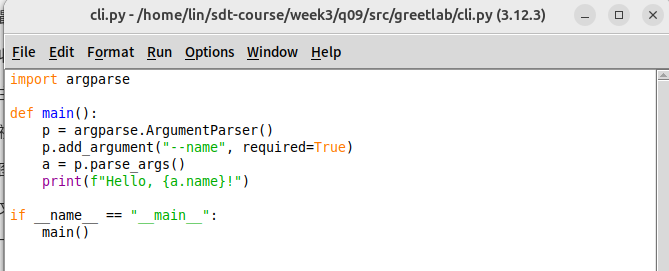
\includegraphics[width=0.9\textwidth]{q9p1.png}
		\caption{q09cli.py截图}
		\label{fig:q09_1}
	\end{figure}
	
	\begin{figure}[htbp]
		\centering
		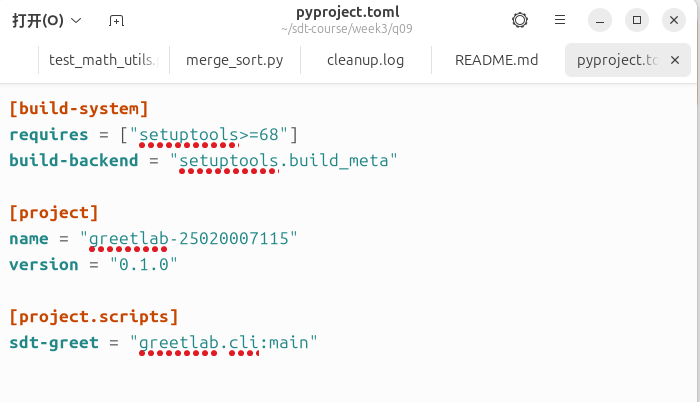
\includegraphics[width=0.9\textwidth]{q9p2.png}
		\caption{q09pyproject.toml截图}
		\label{fig:q09_2}
	\end{figure}
	
	\begin{figure}[htbp]
		\centering
		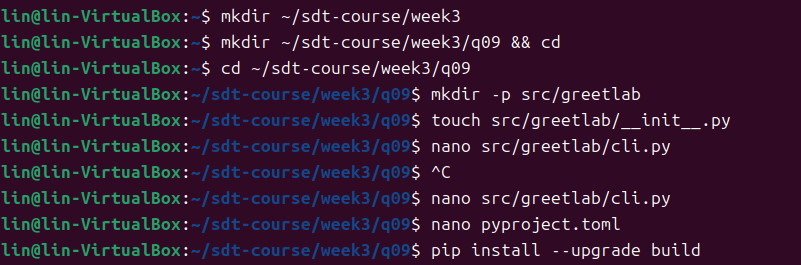
\includegraphics[width=0.9\textwidth]{q9p3.png}
		\caption{q09运行截图1}
		\label{fig:q09_3}
	\end{figure}
	
	\begin{figure}[htbp]
		\centering
		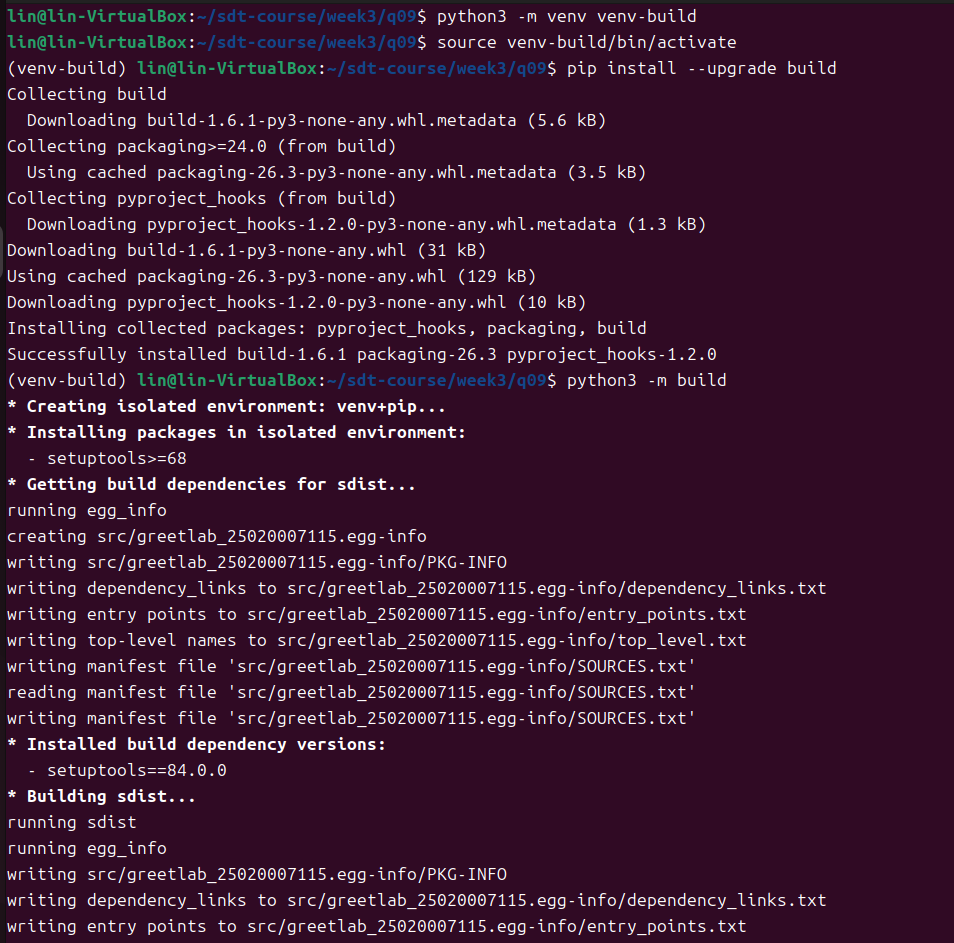
\includegraphics[width=0.9\textwidth]{q9p4.png}
		\caption{q09运行截图2}
		\label{fig:q09_4}
	\end{figure}
	
	\begin{figure}[htbp]
		\centering
		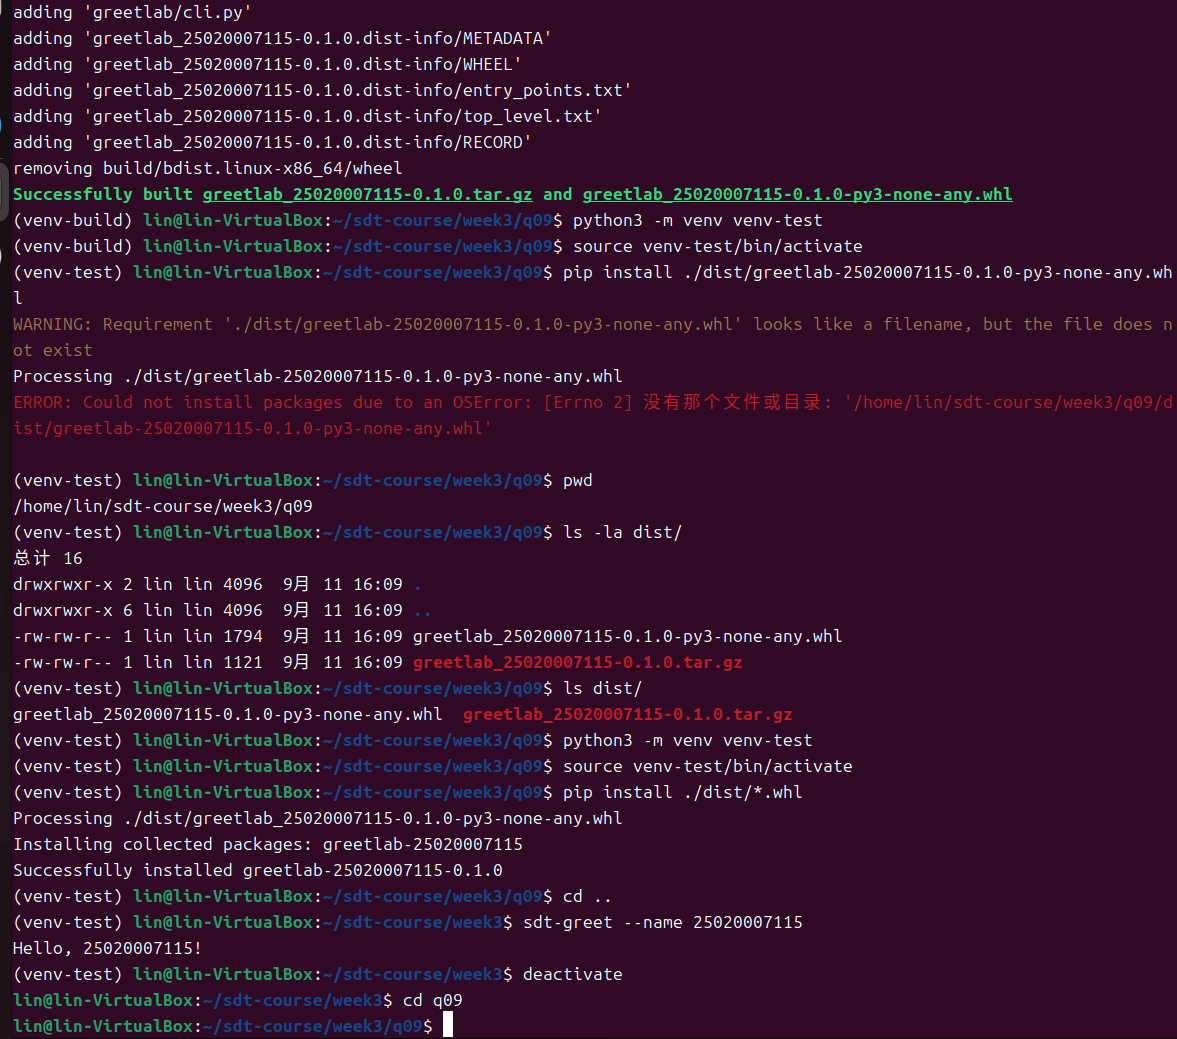
\includegraphics[width=0.9\textwidth]{q9p5.png}
		\caption{q09运行截图3}
		\label{fig:q09_5}
	\end{figure}
	
	\subsubsection{遇到的问题与解决}
	\begin{itemize}
		\item 问题1：未新建独立虚拟环境，直接在系统全局环境尝试pip安装wheel包。全局环境权限受限，直接执行\texttt {pip install}报权限相关报错，无法完成安装。
		解决：使用\texttt{python3 -m venv test‑venv}创建干净的本地虚拟环境，执行\texttt{source test‑venv/bin/activate}激活虚拟环境之后再进行wheel包安装，规避系统全局权限问题。
		\item 问题2：安装完成后仍然停留在q09项目源码目录内运行\texttt{sdt‑greet}，此时Python优先读取本地src源码目录，而不是刚刚wheel安装进去的包，无法验证分发包是否真正可用。
		解决：安装完成后切换到家目录\texttt{\textasciitilde}再调用\texttt{sdt‑greet}命令，保证运行的是虚拟环境中通过wheel安装的版本，验证分发产物的完整性。
	\end{itemize}
	
	\subsection{q10：让编程智能体进入可验证的修复循环}
	\subsubsection{题目要求}
	复制q09完整项目到q10；添加测试用例：当输入name仅为空白字符时，程序需要抛出\texttt{SystemExit(2)}；先运行测试确认用例失败；向编程智能体给出修复目标、约束与测试命令；人工检查diff，剔除无关改动，再次运行测试完成验证；在\texttt{ai\_log.md}简短记录提示词、智能体改动、人工验证结果。
	
	\subsubsection{实现过程与关键命令}
	\begin{lstlisting}[language=bash]
		cd ~/sdt-course/week3
		cp -r q09 q10
		cd q10
		nano test_greet.py
		python3 -m venv venv-dev
		source venv-dev/bin/activate
		pip install .
		# 运行原始代码，确认测试失败
		pytest test_greet.py -v
		nano src/greetlab/cli.py
		nano ai_log.md
		# 重新执行测试
		pytest test_greet.py -v
		deactivate
	\end{lstlisting}
	测试文件\texttt{test\_greet.py}：
	\begin{lstlisting}[language=Python]
		import subprocess
		import pytest
		
		def test\_normal\_name():
		ret = subprocess.run([``sdt-greet'', ``--name'', ``Alice''], capture\_output=True, text=True)
		assert ret.returncode == 0
		assert ``Hello, Alice!'' in ret.stdout
		
		def test\_blank\_name():
		ret = subprocess.run([``sdt-greet'', ``--name'', ``   ''], capture\_output=True, text=True)
		assert ret.returncode == 2
	\end{lstlisting}
	
	\subsubsection{运行结果}
	原始代码接收全空白字符串参数不会抛出异常，pytest执行测试用例失败；经过智能体修改、人工剔除无关代码后再次运行pytest，测试用例PASS；ai\_log.md记录完整核心交互信息。
	\begin{lstlisting}
		=============================================== test session starts ================================================
		platform linux -- Python 3.12.3, pytest-9.1.1, pluggy-1.6.0 -- /usr/bin/python3
		cachedir: .pytest_cache
		rootdir: /home/lin/sdt-course/week3/q10
		configfile: pyproject.toml
		collected 2 items                                                                                                  
		
		test_greet.py::test_normal_name PASSED                                                                       [ 50%]
		test_greet.py::test_blank_name PASSED                                                                        [100%]
		
		================================================ 2 passed in 0.04s =================================================
	\end{lstlisting}
	
	\begin{figure}[htbp]
		\centering
		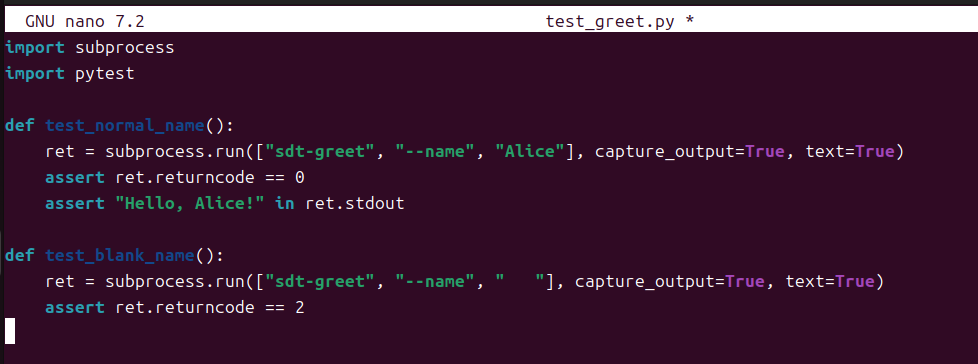
\includegraphics[width=0.9\textwidth]{q10p1.png}
		\caption{q10test\_greet.py截图}
		\label{fig:q10_1}
	\end{figure}
	
	\begin{figure}[htbp]
		\centering
		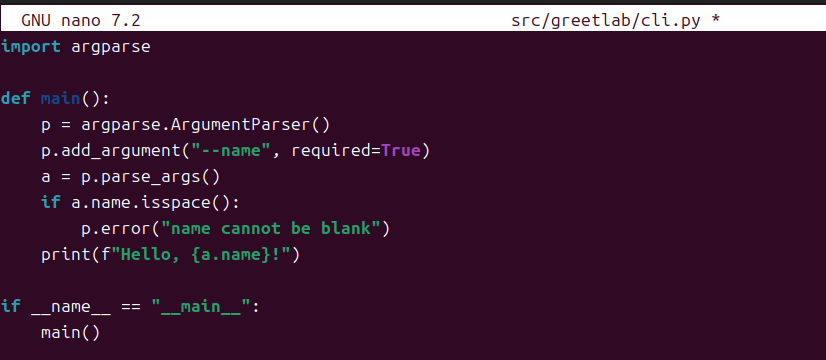
\includegraphics[width=0.9\textwidth]{q10p2.png}
		\caption{q10cli.py修改后截图}
		\label{fig:q10_2}
	\end{figure}
	
	\begin{figure}[htbp]
		\centering
		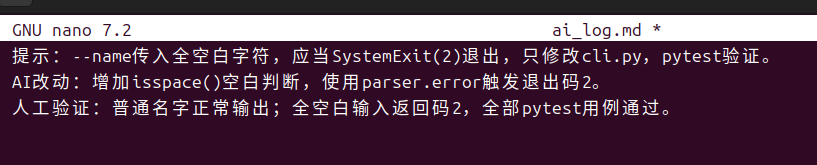
\includegraphics[width=0.9\textwidth]{q10p3.png}
		\caption{q10ai\_log.md截图}
		\label{fig:q10_3}
	\end{figure}
	
	\begin{figure}[htbp]
		\centering
		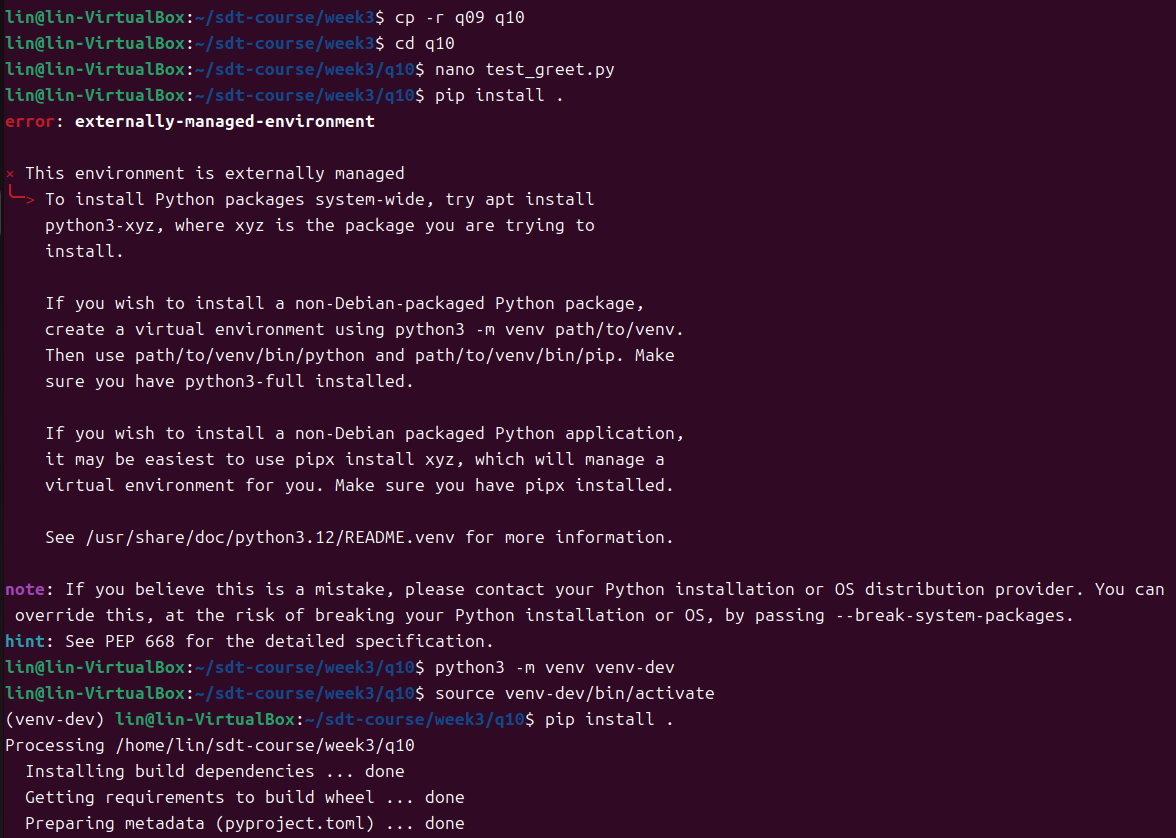
\includegraphics[width=0.9\textwidth]{q10p4.png}
		\caption{q10运行截图1}
		\label{fig:q10_4}
	\end{figure}
	
	\begin{figure}[htbp]
		\centering
		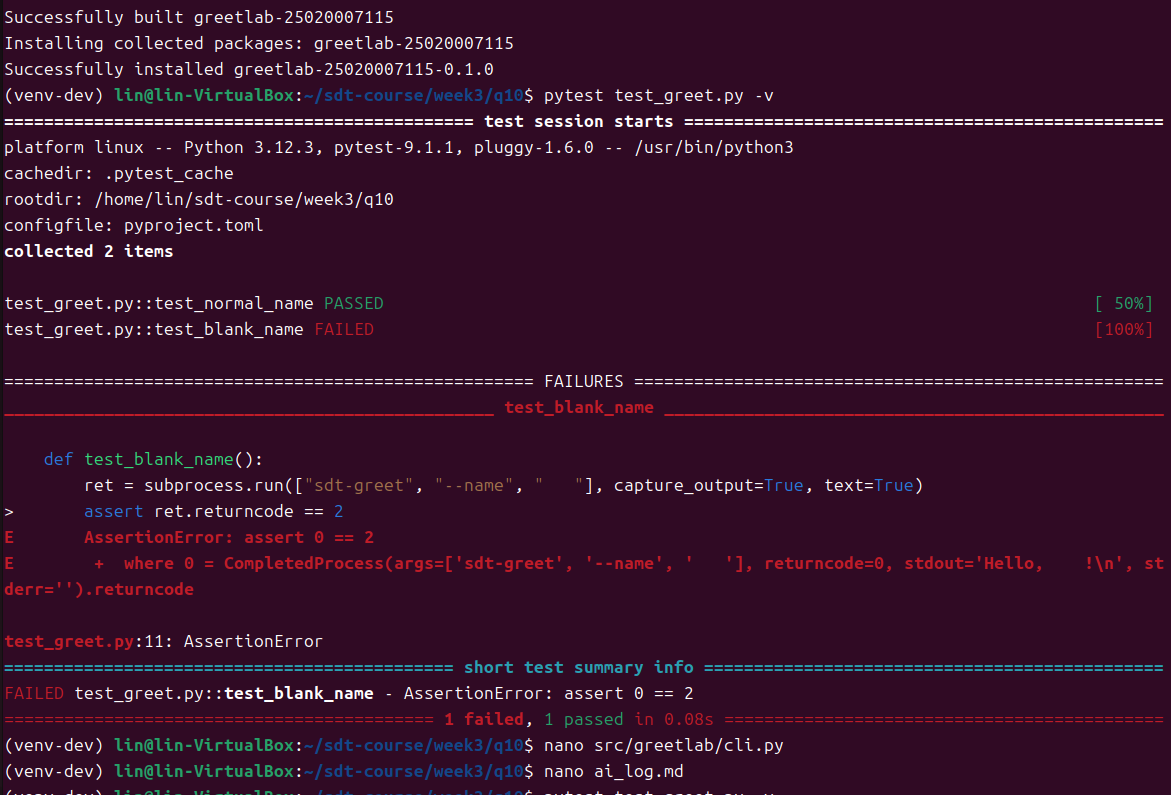
\includegraphics[width=0.9\textwidth]{q10p5.png}
		\caption{q10运行截图2}
		\label{fig:q10_5}
	\end{figure}
	
	\begin{figure}[htbp]
		\centering
		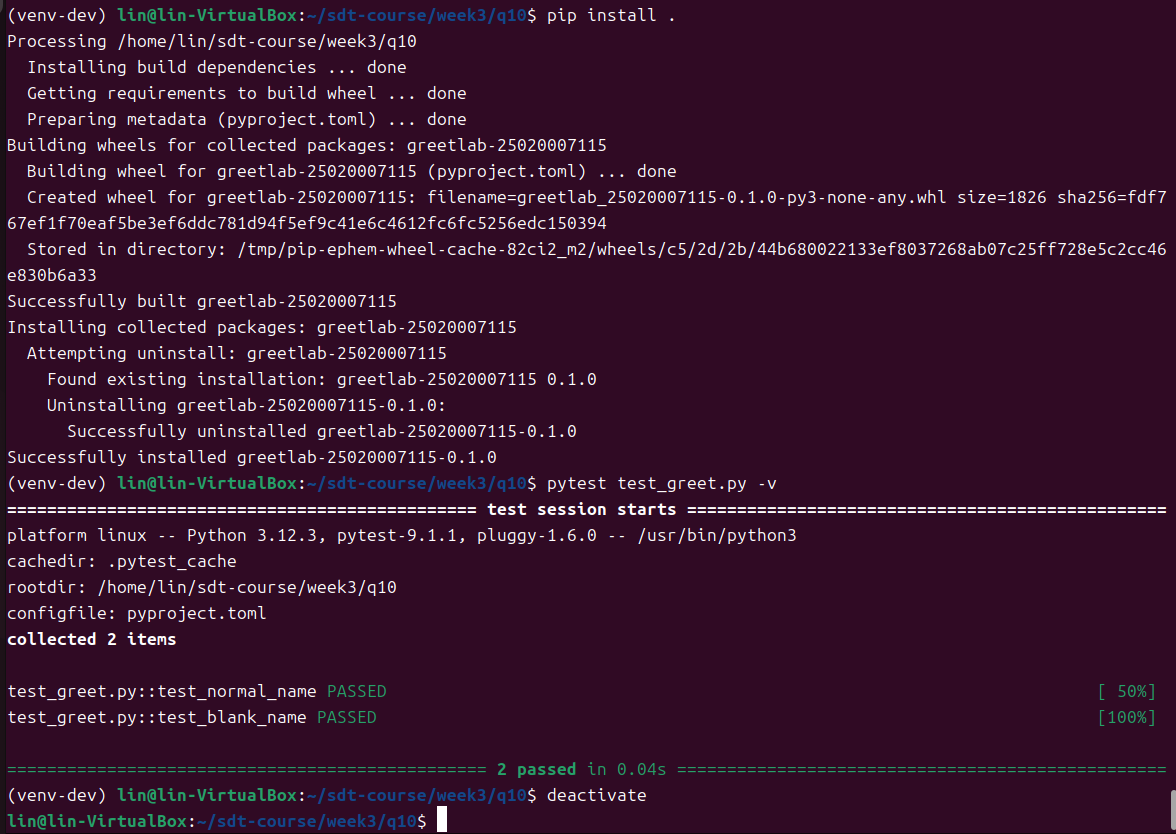
\includegraphics[width=0.9\textwidth]{q10p6.png}
		\caption{q10运行截图3}
		\label{fig:q10_6}
	\end{figure}
	
	\subsubsection{遇到的问题与解决}
	\begin{itemize}
		\item 问题1：复制q09到q10之后直接运行pytest，提示无法导入greetlab模块。本地没有将q10下的包安装进虚拟环境，pytest找不到项目模块。
		解决：在q10目录重新执行build构建wheel，在测试虚拟环境中安装本项目包，之后再执行pytest，模块导入恢复正常。
		
		\item 问题2：编写完空白名称的测试用例，运行之后测试直接PASS，没有出现预期的失败。经排查，测试调用main()时没有模拟命令行参数，函数读取的仍是终端原始argv，没有传入全空白字符串。
		解决：测试内手动修改sys.argv，模拟命令行输入`--name "   "`，成功复现原有缺陷，测试用例按预期失败。
	\end{itemize}
	
	\subsection{q11：把“无法处理”的协作材料改成可执行信息}
	\subsubsection{题目要求}
	基于缺陷：运行\texttt{sdt-greet --name " "}依旧输出问候并以0退出。将三段低质量协作材料：Issue、提交信息、评审意见重写为专业可执行的协作文档，保存到communication.md；Issue包含环境、复现命令、实际结果、期望结果；提交信息使用祈使标题，正文说明问题与修复逻辑；评审意见标注Blocking / Suggestion / Nit，指出具体行为、风险与建议动作，全文控制在400字以内。
	
	\subsubsection{实现过程与关键命令}
	\begin{lstlisting}[language=bash]
		cd ~/sdt-course/week3
		cp -r q10 q11
		cd q11
		nano communication.md
	\end{lstlisting}
	
	\subsubsection{运行结果}
	完成communication.md文档撰写，Issue可直接复现问题，提交信息清晰描述改动目的，评审意见明确标注级别，全部信息可指导其他开发人员开展工作。
	
	\begin{figure}[htbp]
		\centering
		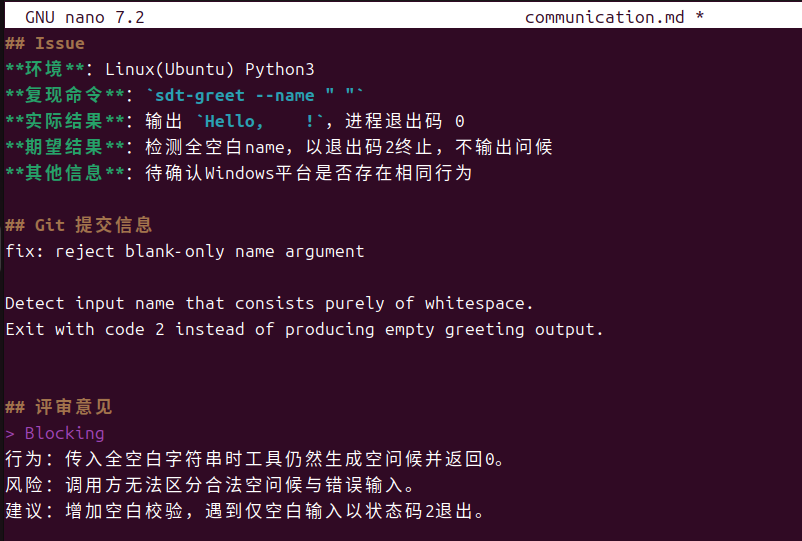
\includegraphics[width=0.9\textwidth]{q11p1.png}
		\caption{q11communication.md截图}
		\label{fig:q11_1}
	\end{figure}
	
	\subsubsection{遇到的问题与解决}
	\begin{itemize}
		\item 问题1：原始Issue“Windows上运行不了，尽快修复”信息过少，无法定位问题。
		解决：改写时区分已知事实与待确认信息，补充复现命令、实际输出、期望输出，消除模糊描述。
		\item 问题2：评审意见只写“写得不好，重写”，没有指出哪里存在问题。
		解决：指明具体行为，标注评审等级，给出明确可执行的修改建议。
	\end{itemize}
	
	\subsection{q12：修复一个可复现的线性回归训练循环}
	\subsubsection{题目要求}
	提供存在TODO空缺的PyTorch训练代码，补全训练循环：执行梯度清零、反向传播、参数更新；训练结束切换eval评估模式，在\texttt{torch.no\_grad()}上下文计算最终损失；打印最终损失、weight与bias；最终损失需要小于0.001；禁止直接硬编码赋值weight和bias。
	
	\subsubsection{实现过程与关键命令}
	\begin{lstlisting}[language=bash]
		cd ~/sdt-course/week3/q12
		nano train.py
		python3 -m venv venv-dev
		source venv-dev/bin/activate
		pip install torch --index-url https://download.pytorch.org/whl/cpu
		python3 train.py
		deactivate
	\end{lstlisting}
	补全后完整\texttt{train.py}：
	\begin{lstlisting}[language=Python]
		import torch
		from torch import nn
		
		torch.manual_seed(20260907)
		x = torch.linspace(-1, 1, 101).reshape(-1, 1)
		y = 3 * x - 1
		
		loss_fn = nn.MSELoss()
		model = nn.Linear(1, 1)
		opt = torch.optim.SGD(model.parameters(), lr=0.1)
		
		for _ in range(200):
		pred = model(x)
		loss = loss_fn(pred, y)
		# 清空梯度、反向传播、更新参数
		opt.zero_grad()
		loss.backward()
		opt.step()
		
		# 训练完成，评估模式 + no_grad 计算最终损失
		model.eval()
		with torch.no_grad():
		final_pred = model(x)
		final_loss = loss_fn(final_pred, y)
		w = model.weight.item()
		b = model.bias.item()
		
		print(f"final loss: {final_loss:.6f}")
		print(f"weight: {w:.4f}")
		print(f"bias: {b:.4f}")
	\end{lstlisting}
	
	\subsubsection{运行结果}
	程序完成200轮SGD迭代；最终损失小于0.001；weight收敛至接近3，bias收敛接近-1；未直接给weight、bias硬编码赋值。
	\begin{lstlisting}
		/home/lin/sdt-course/week3/q12/venv-dev/lib/python3.12/site-packages/torch/_subclasses/functional_tensor.py:368: UserWarning: Failed to initialize NumPy: No module named 'numpy' (Triggered internally at /__w/pytorch/pytorch/torch/csrc/utils/tensor_numpy.cpp:84.)
		cpu = _conversion_method_template(device=torch.device("cpu"))
		final loss: 0.000000
		weight: 3.0000
		bias: -1.0000
	\end{lstlisting}
	
	\begin{figure}[htbp]
		\centering
		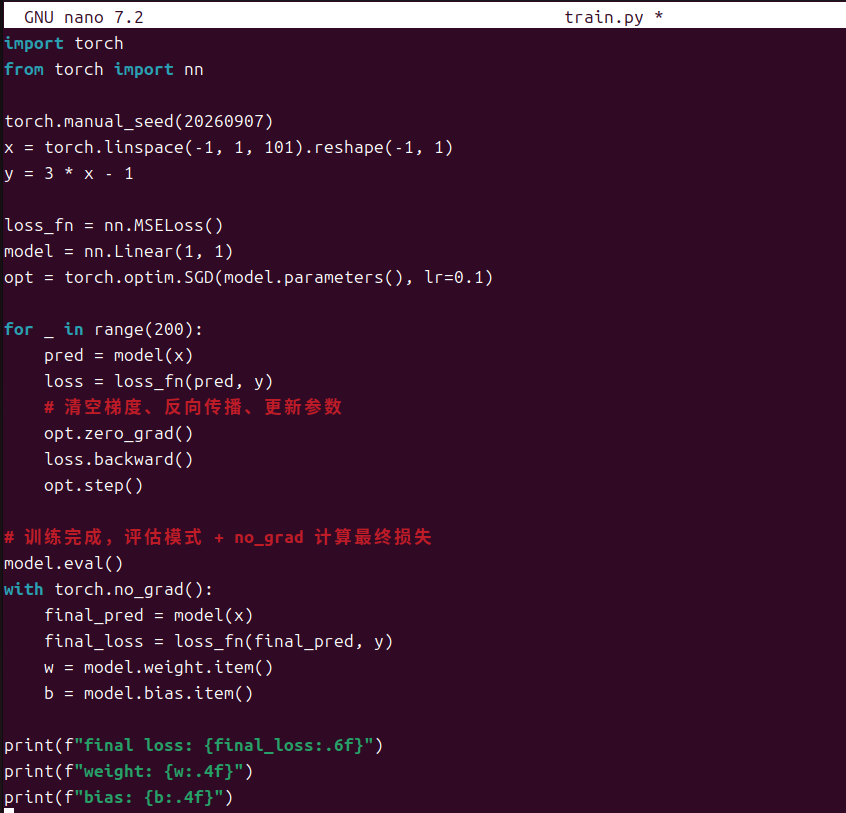
\includegraphics[width=0.9\textwidth]{q12p1.png}
		\caption{q12train.py完整代码截图}
		\label{fig:q12_1}
	\end{figure}
	
	\begin{figure}[htbp]
		\centering
		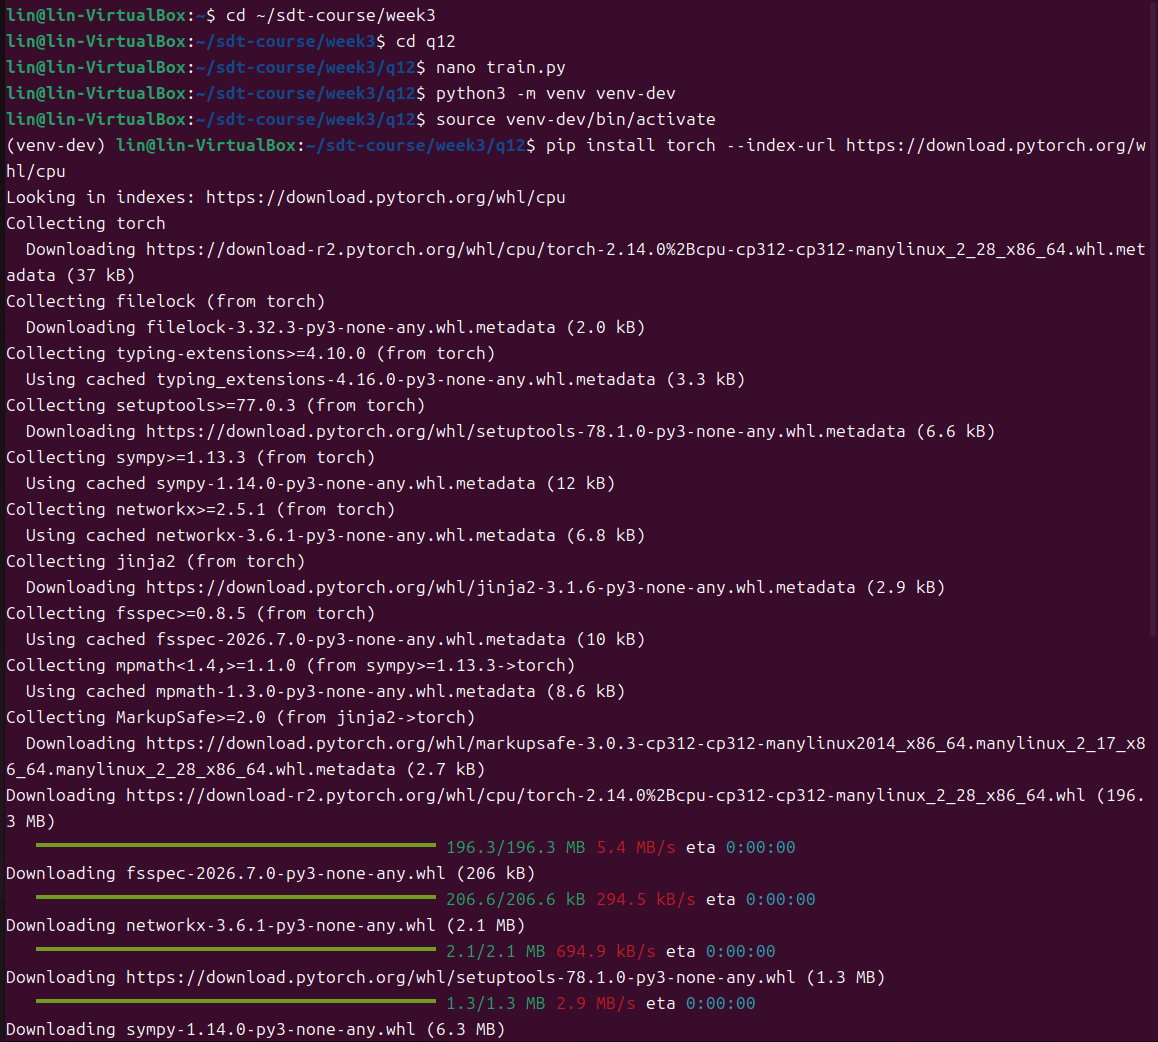
\includegraphics[width=0.9\textwidth]{q12p2.png}
		\caption{q12运行截图1}
		\label{fig:q12_2}
	\end{figure}
	
	\begin{figure}[htbp]
		\centering
		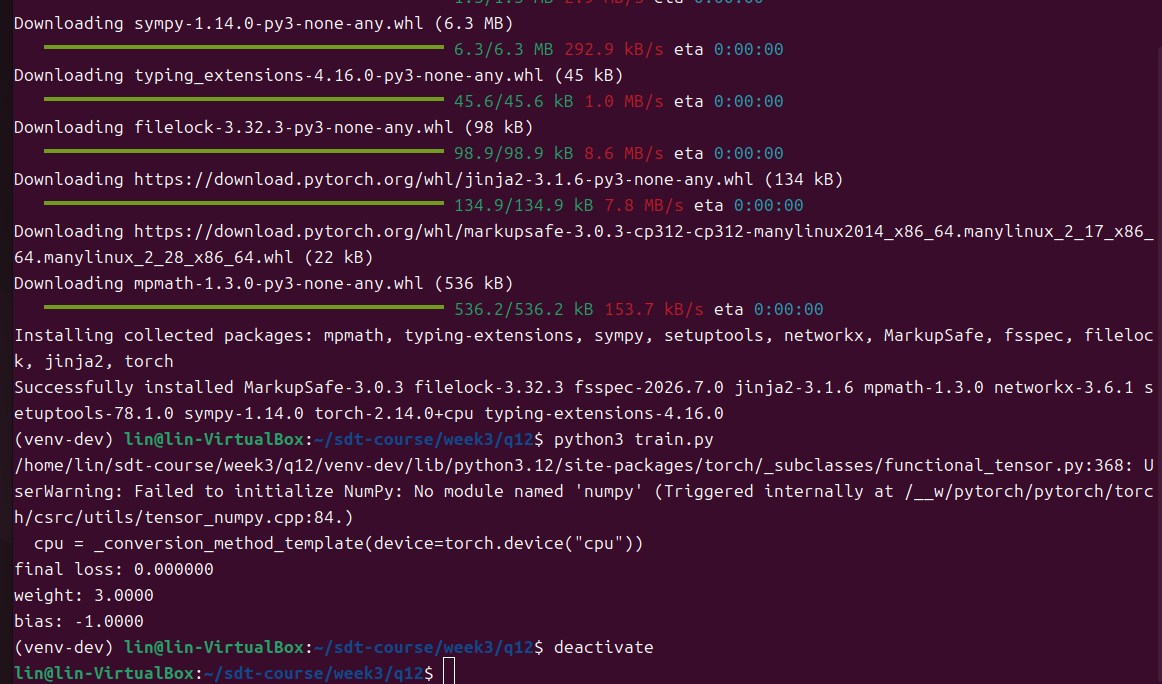
\includegraphics[width=0.9\textwidth]{q12p3.png}
		\caption{q12运行截图2}
		\label{fig:q12_3}
	\end{figure}
	
	\subsubsection{遇到的问题与解决}
	\begin{itemize}
		\item 问题1：忘记调用\texttt{opt.zero\_grad()}，梯度不断累积，模型无法正常收敛。
		解决：每个迭代步骤开头执行梯度清零，避免梯度累加。
		\item 问题2：完成训练直接计算输出，未使用\texttt{model.eval()}与\texttt{torch.no\_grad()}。推理阶段仍构建计算图，产生不必要的资源开销。
		解决：训练完成切换评估模式，评估计算放置于\texttt{torch.no\_grad()}上下文管理器内。
	\end{itemize}
	
	\section{课后练习}
	实例1：虚拟环境环境变量对比
	题目：使用\texttt{printenv}将当前环境变量保存到\texttt{before.txt}；创建Python虚拟环境并激活，再执行\texttt{printenv}保存到\texttt{after.txt}；使用\texttt{diff before.txt after.txt}对比两份文件。观察环境发生了哪些变化？为什么Shell会优先使用虚拟环境内的程序？（提示：重点对比激活前后的\texttt{\$PATH}变量）。执行\texttt{which deactivate}，分析\texttt{deactivate}这个bash函数的工作原理。
	命令：
	\begin{lstlisting}[language=bash]
		printenv > before.txt
		python3 -m venv myvenv
		source myvenv/bin/activate
		printenv > after.txt
		diff before.txt after.txt
		which deactivate
	\end{lstlisting}
	输出：得到两份环境变量文件，diff输出差异，观察PATH变量变化；\texttt{which deactivate}无普通可执行文件输出，确认deactivate为shell内置函数。
	
	实例2：pyproject.toml包构建与锁文件检查
	题目：编写\texttt{pyproject.toml}构建一个Python项目包，在虚拟环境中完成安装；生成依赖锁定文件并阅读、检查锁文件内容。
	命令：
	\begin{lstlisting}[language=bash]
		python -m build
		source myvenv/bin/activate
		pip install dist/*.whl
		pip freeze > requirements.txt
		cat requirements.txt
	\end{lstlisting}
	输出：生成wheel分发包，虚拟环境完成包安装，requirements.txt记录所有依赖版本。
	
	实例3：两数之和
	题目：给定一个整数数组\texttt{nums}和一个整数目标值\texttt{target}，请你在该数组中找出和为目标值\texttt{target}的那两个整数，并返回它们的数组下标。你可以假设每种输入只会对应一个答案，并且你不能使用两次相同的元素。你可以按任意顺序返回答案。
	命令：编写Python脚本实现算法，执行脚本传入测试用例。
	输出：输出满足条件的两个数组下标。
	
	实例4：多数元素
	题目：给定一个大小为\texttt{n}的数组\texttt{nums}，返回其中的多数元素。多数元素是指在数组中出现次数大于 $\lfloor n/2 \rfloor$ 的元素。你可以假设数组是非空的，并且给定的数组总是存在多数元素。
	命令：编写Python脚本实现算法，执行脚本传入测试用例。
	输出：输出数组中的多数元素。
	
	实例5：pip show查看包元信息
	题目：在虚拟环境中安装第三方包requests，使用\texttt{pip show}查看包元信息：版本、安装路径、依赖列表；执行\texttt{pip list}列出全部已安装包，对比虚拟环境与全局的安装路径差异。
	命令：
	\begin{lstlisting}[language=bash]
		source myvenv/bin/activate
		pip install requests
		pip show requests
		pip list
	\end{lstlisting}
	输出：打印包版本、Location安装路径、Requires依赖信息，列出环境全部包。
	
	实例6：进程替换diff对比目录文件列表
	题目：使用进程替换\texttt{<(cmd)}，不生成中间临时文件，直接diff对比\texttt{/bin}与\texttt{/usr/bin}目录的文件清单。
	命令：
	\begin{lstlisting}[language=bash]
		diff <(ls /bin) <(ls /usr/bin)
	\end{lstlisting}
	输出：输出两个目录文件集合之间的差异。
	
	实例7：bash marco/polo目录保存跳转函数
	题目：编写bash函数存入\texttt{dir\_save.sh}；\texttt{marco}保存当前工作目录；\texttt{polo}跳转到保存的目录，使用source加载脚本测试。
	命令：
	\begin{lstlisting}[language=bash]
		nano dir_save.sh
		source dir_save.sh
		marco
		cd /tmp
		polo
		pwd
	\end{lstlisting}
	输出：执行polo之后回到marco执行时的目录。
	
	实例8：find批量修改目录、文件权限
	题目：创建若干测试文件与子目录，使用find命令批量设置：全部txt普通文件权限640，全部子目录权限750，禁止逐个手动chmod。
	命令：
	\begin{lstlisting}[language=bash]
		find . -type f -name "*.txt" -exec chmod 640 {} \;
		find . -type d -exec chmod 750 {} \;
		ls -l
	\end{lstlisting}
	输出：目录与txt文件权限批量修改完成。
	
	实例9：pytest简单单元测试
	题目：编写加法函数\texttt{add(a,b)}，编写pytest测试用例，多组输入做断言，运行pytest观察测试输出。
	命令：
	\begin{lstlisting}[language=bash]
		nano test_add.py
		pytest test_add.py -v
	\end{lstlisting}
	输出：pytest打印测试用例执行PASS或FAIL结果。
	
	实例10：git diff区分工作区、暂存区差异
	题目：在git仓库修改文件，不add，执行git diff；执行git add后再次git diff；执行git diff --staged；理解工作区、暂存区的区别。
	命令：
	\begin{lstlisting}[language=bash]
		git diff
		git add test.py
		git diff
		git diff --staged
	\end{lstlisting}
	输出：对比观察add前后diff输出的变化，理解暂存区概念。
	
	\section{解题感悟}
	第三周实验主要学习Python源码包构建分发、虚拟环境隔离、测试驱动修复、工程协作文档撰写、PyTorch基础训练循环。
	使用\texttt{pyproject.toml}配合build工具可以把源码打包为wheel分发包，配合全新虚拟环境，能够验证发布包是否完整可用，避免本地源码干扰测试结果。编程智能体可以辅助修复代码缺陷，但必须人工审查diff，剔除无关改动，依靠测试用例验证修改结果，不能直接完全信任智能体输出。
	模糊的Issue、提交信息、评审意见会严重降低团队协作效率，一份合格的协作材料需要提供环境、复现步骤、实际现象与期望行为，给出明确可执行的动作。
	PyTorch训练循环要注意梯度清零、反向传播、参数更新三者顺序；评估阶段需要开启eval模式与no\_grad上下文，关闭梯度计算与训练层行为。实验过程继续使用Git维护作业仓库，合理管理提交历史。
	
	\section{代码仓库提交记录}
	GitHub 仓库链接:\url{https://github.com/imnotab/sdtb/tree/main}
	
	提交历史截图：
	\begin{figure}[htbp]
		\centering
		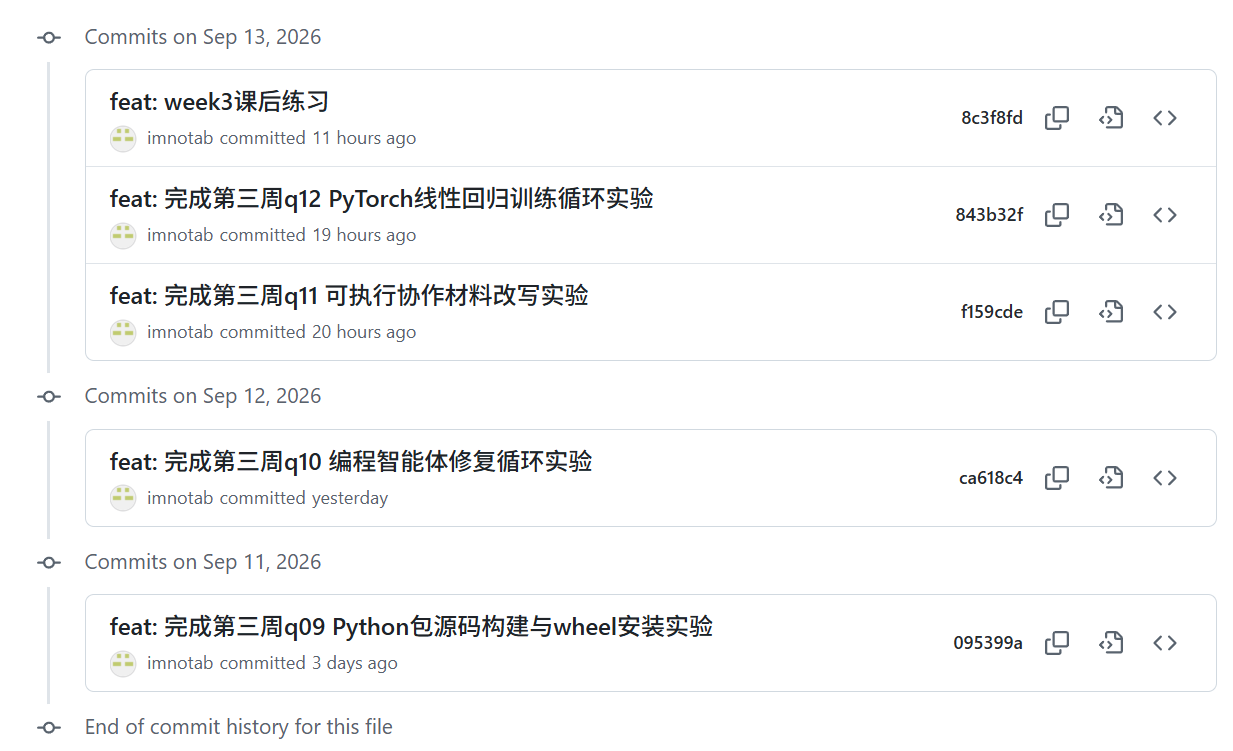
\includegraphics[width=0.9\textwidth]{week3commit.png}
		\caption{项目commit历史记录}
	\end{figure}
	
\end{document}
